Label the sections of the program in memory and describe what is stored in each.

\begin{minipage}{0.2\textwidth}
	%\vspace{-48pt}
	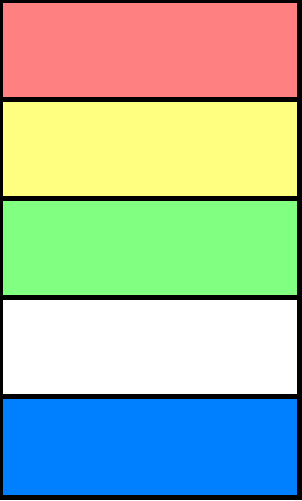
\includegraphics[width=35mm]{other/programstructure.png}
\end{minipage}
%\hspace{50px}
\begin{minipage}{0.7\textwidth}
	\begin{answer}

	\texttt{text} -- machine language version of the source code

	\bigskip \medskip

	\texttt{data} -- global variables

	\bigskip \medskip

	\texttt{heap} -- dynamically allocated storage during program execution

	\bigskip \medskip

	(extra space for the heap and stack to use as needed)

	\bigskip \medskip

	\texttt{stack} -- local variables and the function-calling sequence

	\end{answer}
\end{minipage} \hfill




